%-------------------------
% Resume in Latex
% Author : Sourabh Bajaj
% Website: https://github.com/sb2nov/resume
% License : MIT
%------------------------

\documentclass[11pt]{article}
% \usepackage[a4paper, margin=3in]{geometry}
% \usepackage{geometry}

\usepackage{latexsym}
\usepackage[empty]{fullpage}
\usepackage{titlesec}
\usepackage{marvosym}
\usepackage[usenames,dvipsnames]{color}
\usepackage{verbatim}
\usepackage{enumitem}
\usepackage{lipsum}
\usepackage[pdftex]{hyperref}
\usepackage{fancyhdr}
\usepackage{wrapfig}
\usepackage{graphicx, tikz, geometry}
\usepackage{float}

\newcount\myloopcounter

\newcommand{\repeatit}[2][10]{%
  \myloopcounter0% initialize the loop counter
  \loop\ifnum\myloopcounter < #1 % Test if the loop counter is < #1
  #2%
  \advance\myloopcounter by 1 % 
  \repeat % start again
}

\pagestyle{fancy}
\fancyhf{} % clear all header and footer fields
\fancyfoot{}
\renewcommand{\headrulewidth}{0pt}
\renewcommand{\footrulewidth}{0pt}

% Adjust margins
\addtolength{\oddsidemargin}{-0.950in}
\addtolength{\evensidemargin}{-0.875in}
\addtolength{\textwidth}{1.975in}
\addtolength{\topmargin}{-1.03in}
\addtolength{\textheight}{2.8in}

\urlstyle{same}

\raggedbottom
\raggedright
\setlength{\tabcolsep}{0in}

% Sections formatting
\titleformat{\section}{
  \vspace{-4pt}\scshape\raggedright\large
}{}{0em}{}[\color{black}\titlerule \vspace{-5pt}]

%-------------------------
% Custom commands
\newcommand{\resumeItem}[2]{
  \item\small{
    \textbf{#1}{: #2 \vspace{-2pt}}
  }
}

\newcommand{\resumeSubheading}[4]{
  \vspace{-1pt}\item
    \begin{tabular*}{0.97\textwidth}{l@{\extracolsep{\fill}}r}
      \textbf{#1} & #2 \\
      \textit{} & \textit{\small #4} \\
    \end{tabular*}\vspace{-12pt}
    \textit{\small\begin{minipage}{0.73\textwidth}#3\end{minipage}}
    \vspace{-5pt}
}

\newcommand{\resumeSubItem}[2]{\resumeItem{#1}{#2}\vspace{-4pt}}

\renewcommand{\labelitemii}{$\circ$}

\newcommand{\resumeSubHeadingListStart}{\begin{itemize}[leftmargin=*]}
\newcommand{\resumeSubHeadingListEnd}{\end{itemize}}
\newcommand{\resumeItemListStart}{\begin{itemize}}
\newcommand{\resumeItemListEnd}{\end{itemize}\vspace{-5pt}}

%-------------------------------------------
%%%%%%  CV STARTS HERE  %%%%%%%%%%%%%%%%%%%%%%%%%%%%


\begin{document}

%----------HEADING-----------------
\begin{tabular*}{\textwidth}{l@{\extracolsep{\fill}}r}
  \textbf{\href{https://github.com/willthbill}{\Large William Bille Meyling}} & E-mail : \href{mailto:williambillemeyling@gmail.com}{williambillemeyling@gmail.com}\\
  \textbf{Github}: \href{https://github.com/willthbill}{https://github.com/willthbill}; \textbf{LinkedIn}: \href{https://bit.ly/linkedin-wbm}{https://bit.ly/linkedin-wbm} & Mobile : +45 24445317 \\
\end{tabular*}

%-----------BIO-----------------
\begin{tikzpicture}[overlay,remember picture]
 \node[anchor=north west,inner sep=0pt]at ([xshift=15.94cm,yshift=-1.8cm]current page.north west) {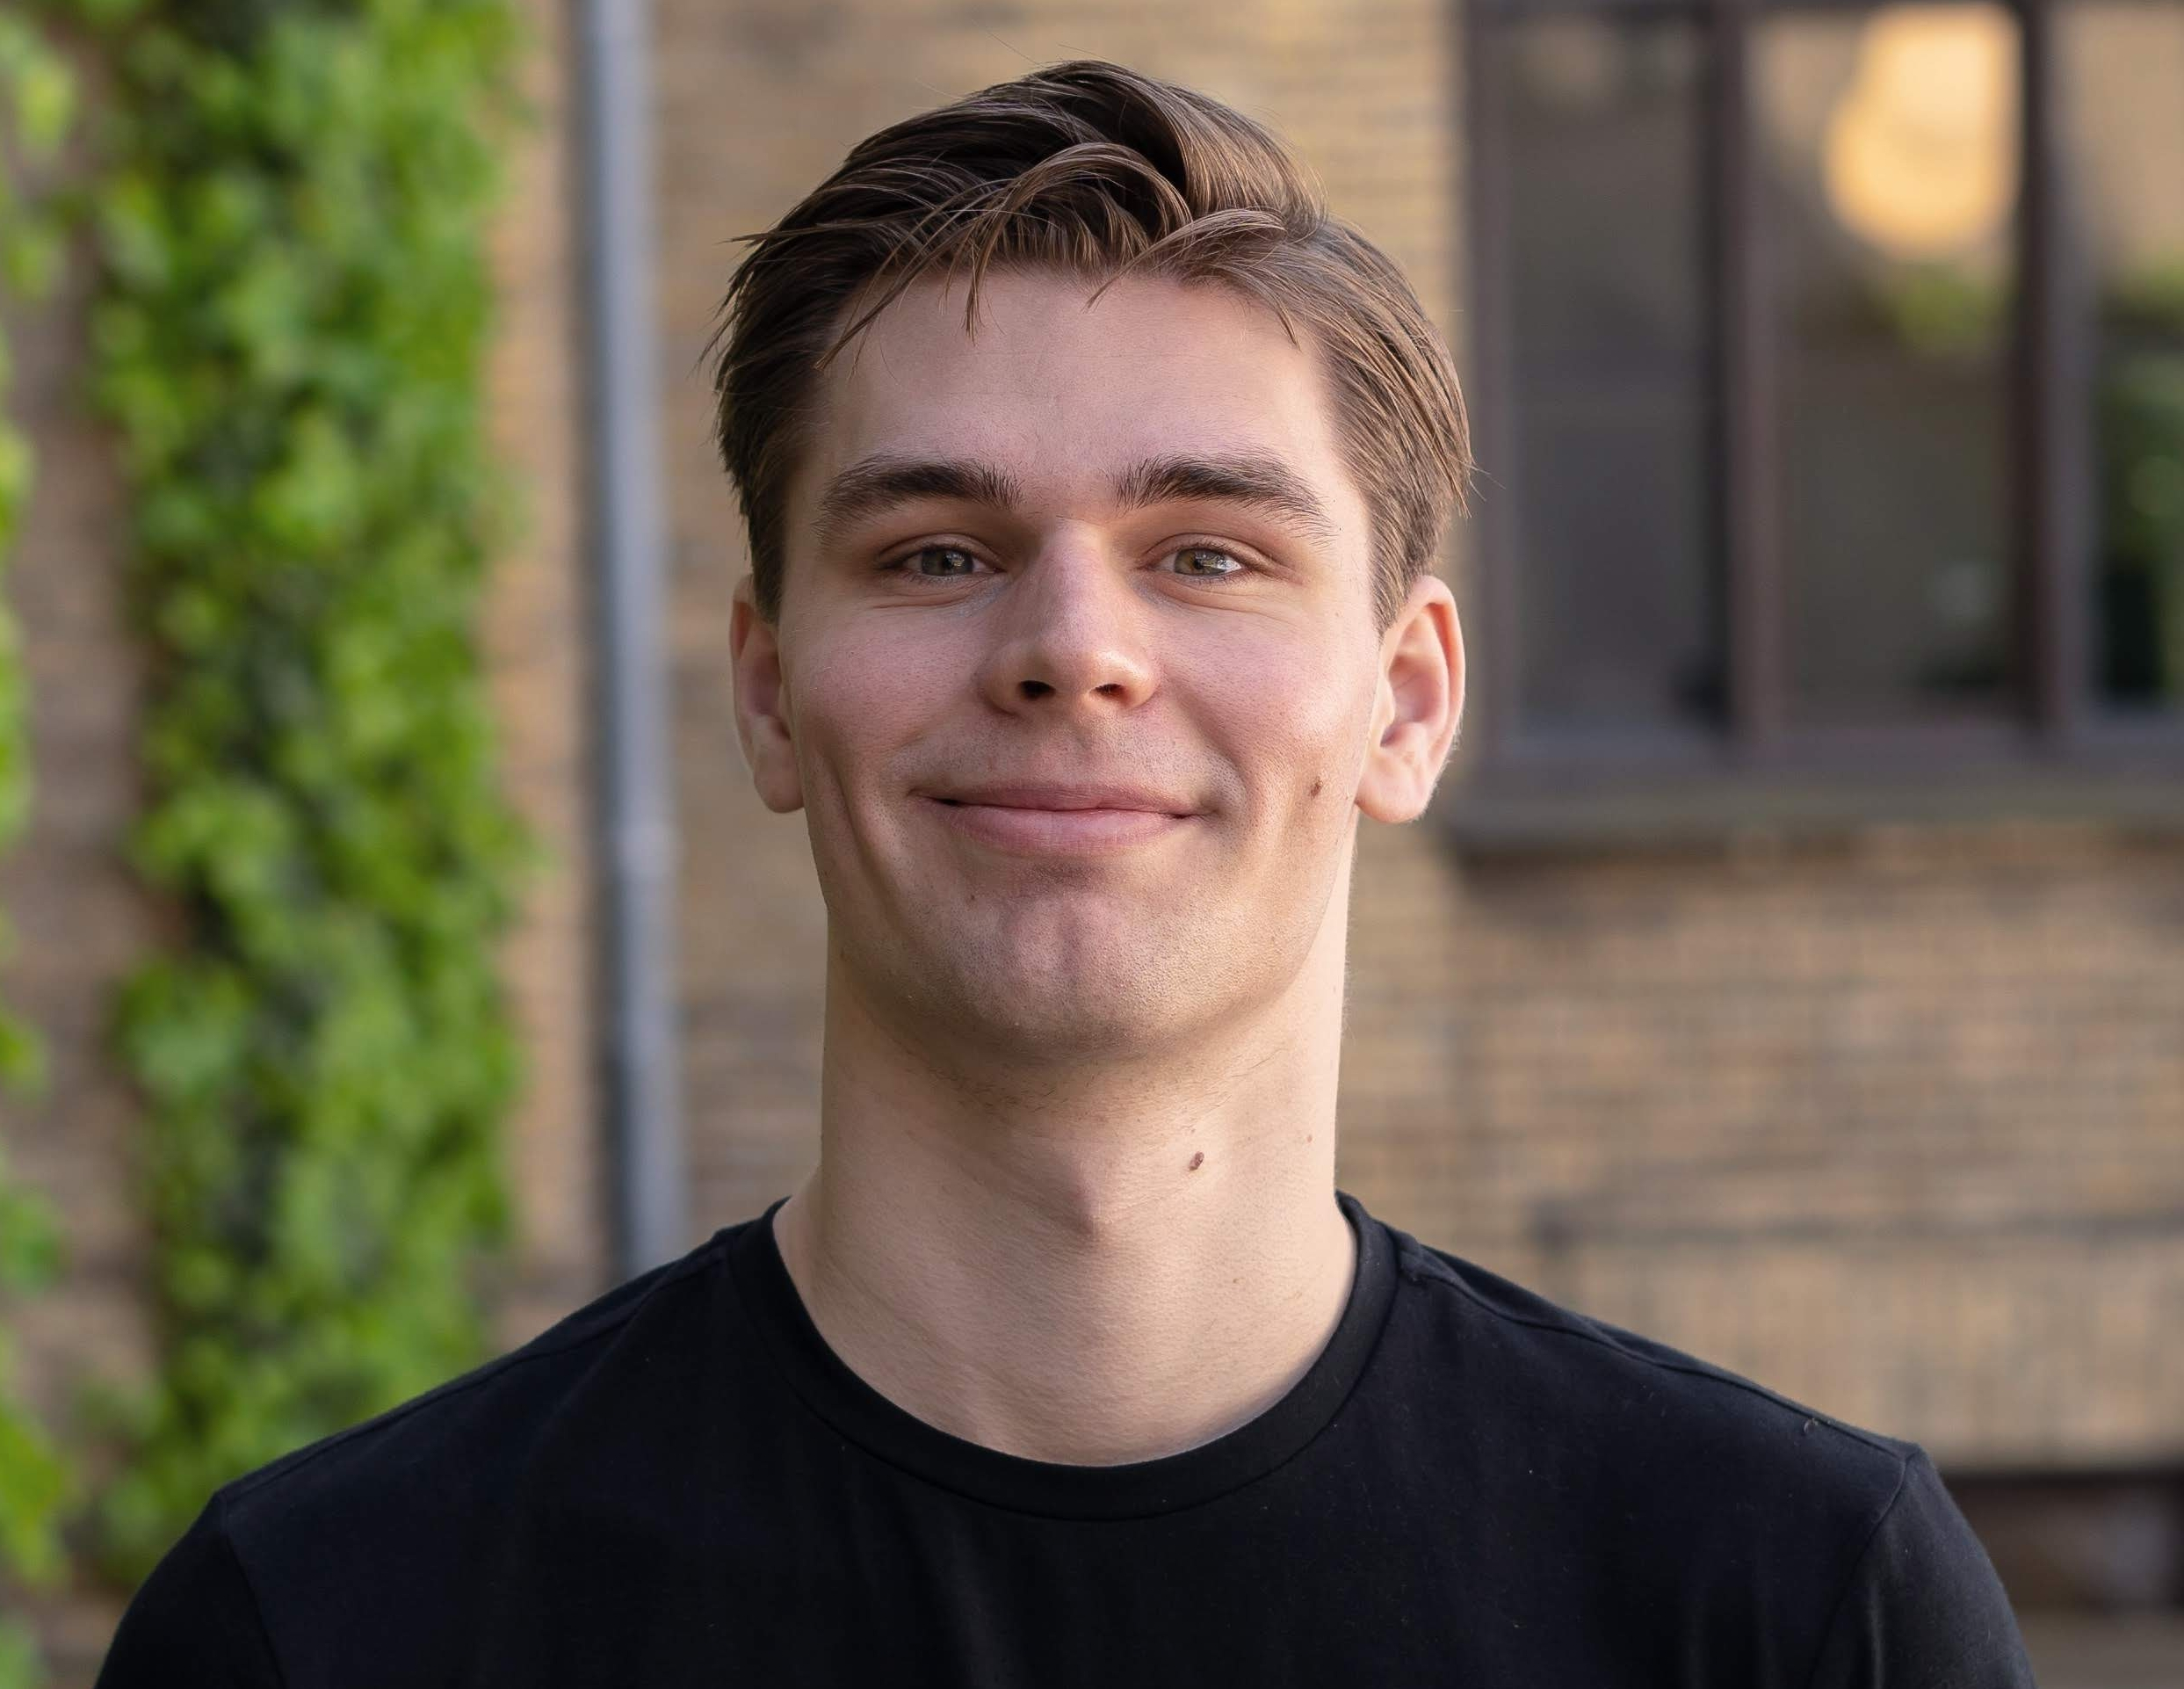
\includegraphics[width=5cm]{me_cropped.jpg}};
\end{tikzpicture}

\begin{minipage}{14.8cm}
A friendly 22 year old Computer Science student with a passion for Algorithm Engineering -- especially within Computational Geometry and Graph Algorithms. I have spend the past 8 years finding and pursuing my interests, winning numerous national and international competitions along the way. I see myself as an innovative person, who appreciates simple solutions to complicated problems. My attention to detail, systematic mindset and curiosity makes me good at planning and quickly building large projects, making few mistakes along the way. My native language is Danish.
\end{minipage}
\vspace{-5pt}

%-----------EDUCATION-----------------
\section{Education}
  \resumeSubHeadingListStart
    \resumeSubheading
      {University of Copenhagen}{Copenhagen, Denmark}
      {Bachelor in Computer Science. Grade: 12}{Sep. 2020 -- Aug. 2023}
    \resumeSubheading
      {Courses in Algorithms and Cybersecurity}{Denmark}
      {DDD training camps and DDC Cybersecurity courses}{Sep. 2018 -- May. 2022}
    \resumeSubheading
      {NEXT Sukkertoppen Gymnasium}{Copenhagen, Denmark}
      {High school. Computer Science and Math. GPA: 11.8}{Aug. 2016 -- Jun. 2020}
  \resumeSubHeadingListEnd
  
%-----------EXPERIENCE-----------------
\section{Experience}
  \resumeSubHeadingListStart
    \resumeSubheading
      {University of Copenhagen}{Copenhagen, Denmark}
      {Teaching assistant in the course 'Algorithms and Data structures'}{Feb. 2023 - Mar. 2023}
    \resumeSubheading
      {Jobindex}{Copenhagen, Denmark}
      {Full-stack Developer. Tools: MySQL, Perl, Vue.js}{Feb. 2021 - Jan. 2022}
    \resumeSubheading
      {Dansk Datalogi Dyst (Danish National Olympiad in Informatics)}{Denmark, Indonesia, Germany}
      {Volunteer. Designing algorithmic problems used to select students for the national team. Training the national team for the International Olympiad in Informatics (IOI). Preparing courses in advanced (beyond bachelor-level) algorithmic techniques. Deputy leader at IOI 2022. \textbf{Vice chairman} of the technical committee of BOI 2023 (International Competition) (\textbf{with salary}).}{Oct. 2020 - present}
    \resumeSubheading
      {Arnvind Group}{Copenhagen, Denmark}
      {Frontend Developer. Tools: React. Responsible for a large complicated wep-app.}{Apr. 2019 - Mar. 2020}
  \resumeSubHeadingListEnd

%-----------AWARDS-----------------
\section{Awards and Achievements}
  \resumeSubHeadingListStart
  
    \resumeSubheading
      {Winner of Computational Geometry Challenge 2023}{Online and in Dallas, Texas}
      {"Unofficial World Championships in Geometric Algorithms" -- a research competition called CG:SHOP. Qualified me for SoCG (the most prestigious Computational geometry conference). Media coverage in \href{https://bit.ly/p1-wbm23}{DR:P1}, \href{https://bit.ly/eb-wbm23}{Ekstra-Bladet}, \href{https://bit.ly/videndk-wbm23}{videnskab.dk} and more. Statement at \href{https://bit.ly/scienceku-wbm23}{https://bit.ly/scienceku-wbm23}}{Sep. 2022 -- Jun. 2023}

    \resumeSubheading
      {Winner of Unge Forskere 2020}{Copenhagen, Denmark (remote)}
      {Danish National Youth Research Championships 2020. Project about Efficient Graph-based Image-segmentation. Media coverage in DR:P1, DR:P3, \href{https://bit.ly/jp-wbm20}{Jyllands-posten}, \href{https://bit.ly/videndk-wbm20}{videnskab.dk} and more. Statement at \href{https://bit.ly/ungefor-wbm20}{https://bit.ly/ungefor-wbm20}}{Apr. 2020}
      
    \resumeSubheading
      {Winner of Danish Programming Championships 2023}{Denmark, Netherlands and Online}
      {Competitive Programming. 4th in 2020, 2nd in 2021, 3rd in 2022, 1st in 2023 (and 3rd in Scandinavia). Qualified for NWERC all four years (Northwestern Europe Regional Contest).}{Nov. 2020 -- present}
      
    \resumeSubheading
      {'Best Computational Project' at European Science Championships}{Salamanca, Spain (remote)}
      {Unge Forskere project received the PRACE Award at EUCYS 2020. Statement at \href{https://bit.ly/prace-wbm21}{https://bit.ly/prace-wbm21}}{Sep. 2021}
      
    \resumeSubheading
      {Top 52\% at the International Olympiad in Informatics (IOI) 2020}{Singapore (remote)}
      {Competitive Programming. IOI participant in 2019 and 2020. Also participated in Baltic Olympiad in Informatics in 2019 and 2020.}{Apr. 2019 - Sep. 2020}

    \resumeSubheading
      {2nd place at Danish AI Championships 2022}{Copenhagen, Denmark}
      {AI Engineering Competition}{Oct. 2022}
      
    \resumeSubheading
      {Winner of Danish National Olympiad in Informatics 2019 and 2020}{Denmark}
      {Dansk Datalogi Dyst. Competitive Programming. Part of the National Team.}{Apr. 2019 -- Sep. 2020}

    \resumeSubheading
      {Master Title on CodeForces}{Online}
      {Competitive Programming. Top 1600 in the world. \href{https://bit.ly/cf-wbm}{https://bit.ly/cf-wbm}}{Sep. 2021 -- present}

    \resumeSubheading
      {Next Generation Award 2020 (Skau Reipurth)}{Copenhagen, Denmark}
      {Given "as an acknowledgement of his talent, hard work and passion for programming". \href{https://bit.ly/skau-wbm20}{https://bit.ly/skau-wbm20}}{Nov. 2020}
      
    \resumeSubheading
      {Finalist in the Danish Cyber Championships 2022}{Copenhagen, Denmark}
      {De Danske Cybermesterskaber 2022. Cybersecurity (CTF) Competition.}{May. 2022}

  \resumeSubHeadingListEnd


%-----------PROJECTS-----------------
\section{Projects \& Publications}
  \resumeSubHeadingListStart
    \resumeSubItem{ExtensionCC}
      {An efficient Convex Cover algorithm developed for CG:SHOP 2023. \\Publication: \href{https://bit.ly/SoCGpub-wbm23}{https://bit.ly/SoCGpub-wbm23}. Bachelor-thesis: \href{https://bit.ly/ba-wbm}{https://bit.ly/ba-wbm}}
    \resumeSubItem{Universal Autonomous Graph-based Image Segmentation with Near-linear Average Complexity}{Unge Forskere project. See more at \href{https://bit.ly/eucys-wbm}{https://bit.ly/eucys-wbm}}
    \resumeSubItem{Pacup}{Open-source tool unifying Linux package managers and making systems reproducible: \href{https://bit.ly/pacup-wbm}{https://bit.ly/pacup-wbm}}
    \resumeSubItem{Opener.nvim}{Open-source Neovim plugin for workspace / context switching: \href{https://bit.ly/opener-nvim}{https://bit.ly/opener-nvim}}
    \resumeSubItem{Codify}{Chrome extension with over 10000 installations.}
  \resumeSubHeadingListEnd

%
%--------PROGRAMMING SKILLS------------
\section{Skills \& Interests}
  \resumeSubHeadingListStart
     \resumeSubItem{Theoretical Computer Science}{Graph algorithms, Computational Geometry, Software Design, AI}
     \resumeSubItem{Favorite Programming Languages}{C++, Python, JavaScript, C, Rust}
     \resumeSubItem{Other}{Linux, DevOps, Web development, Cybersecurity, Automation, Latex, Video editing}
 \resumeSubHeadingListEnd
 
%--------PROGRAMMING SKILLS------------
\section{References}
  \resumeSubHeadingListStart
      \item\small{
        \textbf{Mikkel Vind Abrahamsen (Bachelor supervisor)}{
            \\\hspace{10pt}\textit{E-mail}: miab@di.ku.dk\\\hspace{10pt}\textit{Mobile}: +45 20787534
        \vspace{-2pt}}
      }\vspace{-4pt}
 \resumeSubHeadingListEnd

%-------------------------------------------
\end{document}
